\newpage
\section{Results and Evaluation}
\subsection{Experiment Setup}
The experiment is completed with a 3.1 GHz Intel Core i5 Processor with 8GB of memory. The four implemented encoding schemes were first compared using the size of CNF it generated. Then the encoded results were fed into the model counter miniC2D, and this model counter was selected because it's one of the newest model counting tool available and according to \cite{minic2d}, it outperforms many of the model counting tools. Number of Clauses in the CNF is used in the evaluation because it size of the CNF directly influences the model counting time. Besides, some of the data we gained from the output of the model counter is also compared including Compiling time, Compile memory, and model counting time.\\

\noindent Since the comparison is mainly runtime, to eliminate the variance, each model counting for an encoded benchmark was done five times and took the average. The time limit is 2 hours maximum. The runtime for Full encoding was omitted because, for most of the benchmarks we used, the model counter fails to output result within a reasonable amount of time.\\

\noindent In the experiments and results, we first compare the number of clauses generated by Full encoding and Simplified Full encoding to show the improvement done by encoding determinism, which was mentioned in the previous section that leads to the most significant reduction in the number of clauses and compiling time. Then we compare the size of the CNF generated by Simplified encoding, Improved encoding, and Group encoding.

\subsection{Data}
The experiment data mainly consists of 450 Grid Networks from the the Rochester University Bayesian repository, available in 
\footnote{https://www.cs.rochester.edu/u/kautz/Cachet/Model\_Counting\_Benchmarks/Grid.zip}, as well as the real Bayesian Network files available in \textit{bnlearn} repository \footnote{http://www.bnlearn.com/bnrepository/}. Table \ref{tab:benchmark_info} shows the detail information about the experiment data.\\

\noindent The grid networks are in size N $\times$ N, with a deterministic ratio $R$ specifying the scale of deterministic, which means the number of nodes whose values are determined given the values of their parents. \\

\begin{table}[]
    \centering
    \begin{tabular}{l p{5cm}}
    \hline
    Netorks	&	Information	\\
    \hline
    \hline
    Ratio 50	&	Contains 90 networks with nodes from 10 $\times$ 10 to  20 $\times$ 20 	\\
    \hline
    Ratio 75	&	Contains 150 networks with nodes from 10 $\times$ 10 to  26 $\times$ 26 	\\
    \hline
    Ratio 90	&	Contains 210 networks with nodes from 10 $\times$ 10 to  50 $\times$ 50  \\
    \hline
    \end{tabular}
    \caption{Benchmark information}
    \label{tab:benchmark_info}
\end{table}


\noindent The dataset is chosen because Weighted model counting method performs well on highly deterministic Bayesian Networks and the Ratio indicates the deterministic extend that helps the result analysis.

\subsection{Encoding determinism}
The Simplified Full Encoding captures the determinism and simplifies the encoded results compared to the Full encoding. Some of the results are shown in Table \ref{tab:enc-determin}. The results indicate that the simplification leads to a significant reduction in both the number of variables and size of the CNF. Larger deterministic ratio leads to a larger reduction. The average reduction for Ratio\_50, Ratio\_75 and Ratio\_90 are 48.43\%, 67.09\% and 80.06\% respectively. The the visualization of the result is given in figure \ref{fig:determinism}.

\begin{table}[]
    \centering
    \begin{tabular}{c c | c c  c c c }
        \hline
        &	&	Full enc	&	Simplified 	&	Full enc & Simplified &	Average\\
        Ratio & N	&   Var Num	&   Var Num	&	clause Num	& clause Num & 	Reduction\\
        \hline
        \hline
                &12	&	1346 	& 	614	&	 4428 	&	2126 &	\\
                &14	&	1850 	&	906	&	 6116 	&	3158 &	 \\
        Ratio 50&16	&	2434    &	1186	&	 8076 	&	4156 &	48.43\%\\
                &18	&	3098    &	1494	&	 10308 	&	5260 &	\\
                &20	&	3842 	&	1826	&	 12812 	&	6428 &	\\
        \hline
                &10	&	922	    &	266	&	3012	&	918 &	\\
                &12	&	1346	&	458	&	4428	&	1608 &	\\
       Ratio 75 &14	&	1850	&	458	&	6116	&	1614 & 67.09\%	\\
                &15	&	2132	&	635	&	7062	&	2240 &	\\
                &16	&	2434	&	738	&	8076	&	2612 &	\\
        \hline
                &10	&	922	    &	178	&	3012	&	618	& \\
                &12	&	1346	&	266	&	4428	&	944	& \\
        Ratio 90&14	&	1850	&	346	&	6116	&	1238 & 80.06\%	\\
                &15	&	2132	&	487	&	7062	&	1742 &	\\
                &16	&	2434	&	366	&	8076	&	1338 &	\\
        \hline
        \hline
    \end{tabular}
    \caption{Comparing number of clauses and numbers of variables before and after encoding determinism. N indicates the size of the Grid Network}
    \label{tab:enc-determin}
\end{table}

 
\begin{figure}[h]
\centering
\begin{subfigure}{0.32\textwidth}
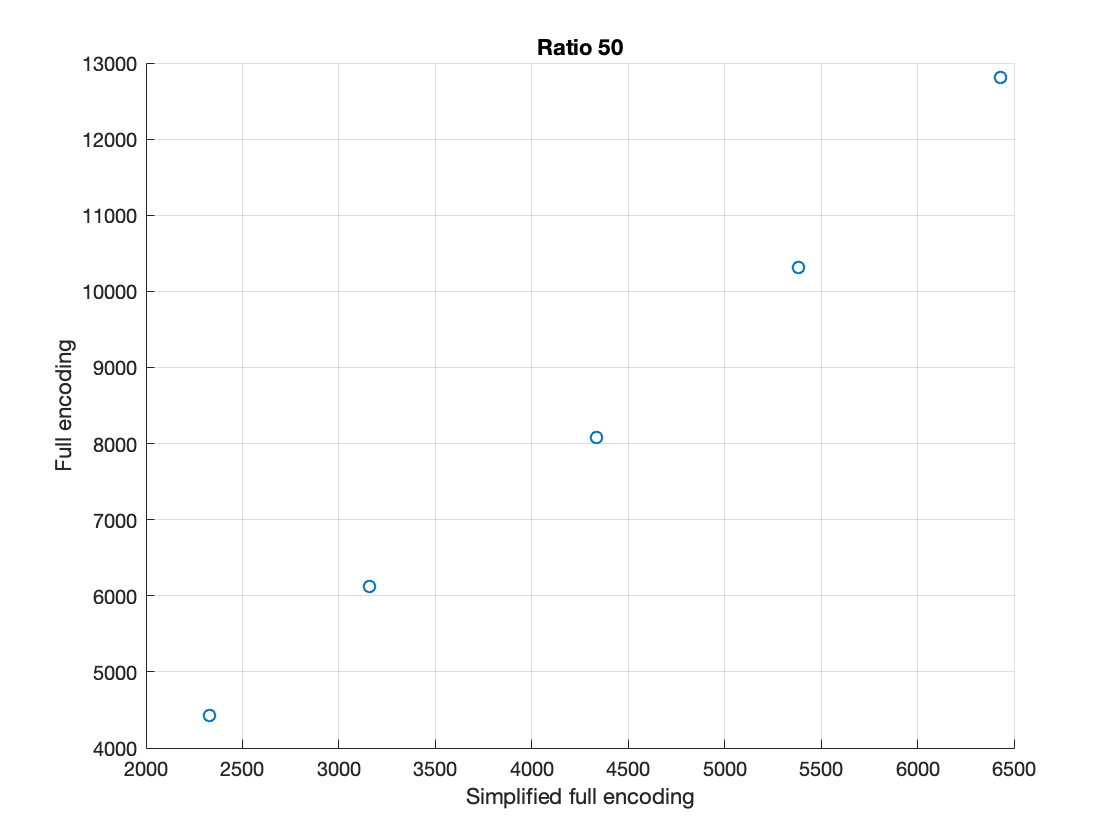
\includegraphics[width=0.9\linewidth]{pic/r50_determinism.png}
\caption{Ratio 50 determinism}
\label{fig: r50_determin}
\end{subfigure}
\begin{subfigure}{0.32\textwidth}
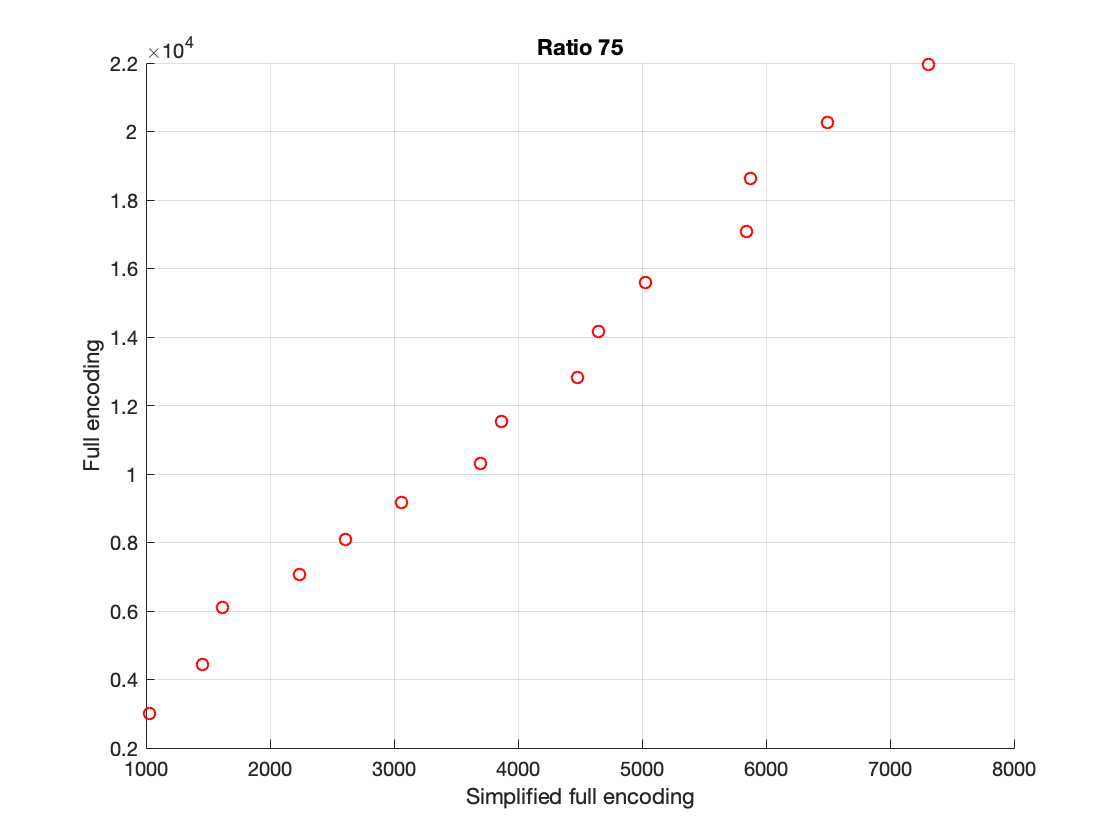
\includegraphics[width=0.9\linewidth]{pic/r75_determinism.png}
\caption{Ratio 75 determinism}
\label{fig: r75_determin}
\end{subfigure}
\begin{subfigure}{0.32\textwidth}
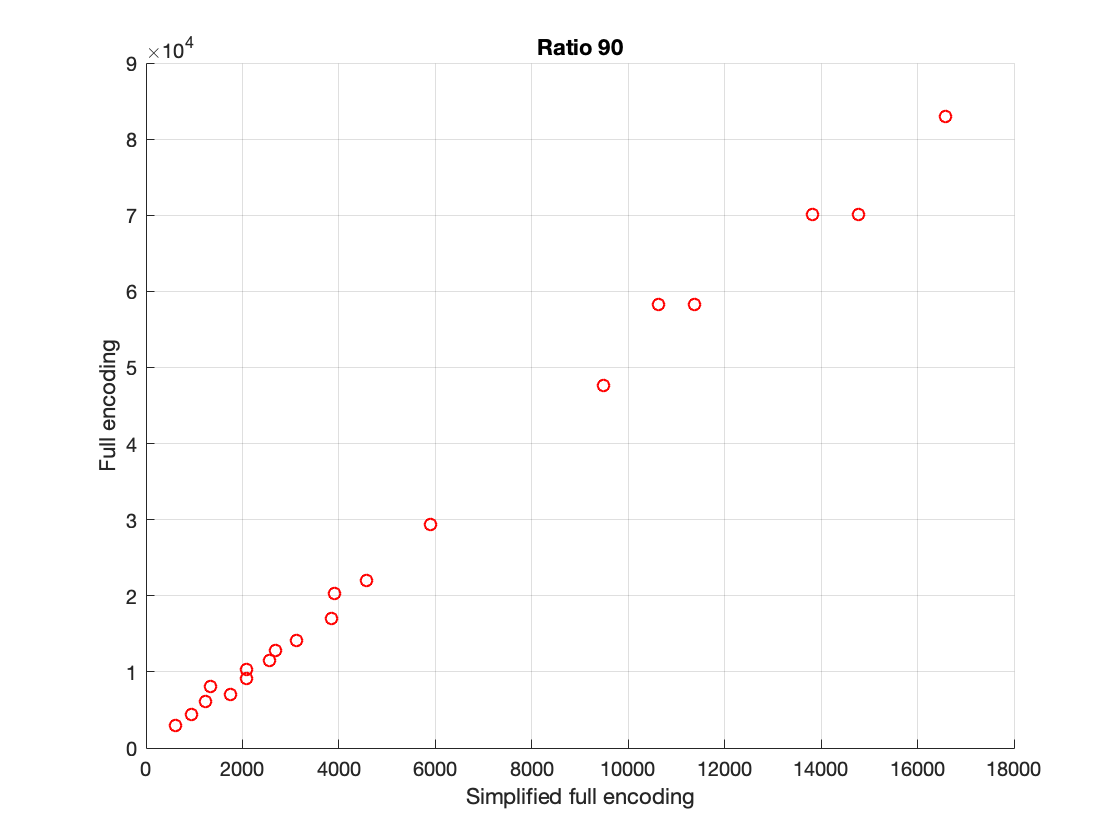
\includegraphics[width=0.9\linewidth]{pic/r90_determism.png}
\caption{Ratio 90determinism}
\label{fig: r90_determin}
\end{subfigure}
 
\caption{Full encoding vs Simplified encoding}
\label{fig:determinism}
\end{figure}

\subsection{Number of Clauses}
Table \ref{tab:comparing the clauses} shows the group of networks three groups of networks from the repository to evaluate the three encoding schemes. Comparing the first and second row indicates that with regard of the size of encoded CNF file, in general, Improved encoding is better than the Simplified encoding while the reduction is not that significant when comparing Improve Encoding and Group Encoding. However, even though the size is not significantly reduced, through pre-processing the CNF to make use of the semantically independent components, the model counting and compiling time as well as the file size was reduced considerably. This is discussed later in the following paragraphs.\\
\begin{figure}
    \centering
    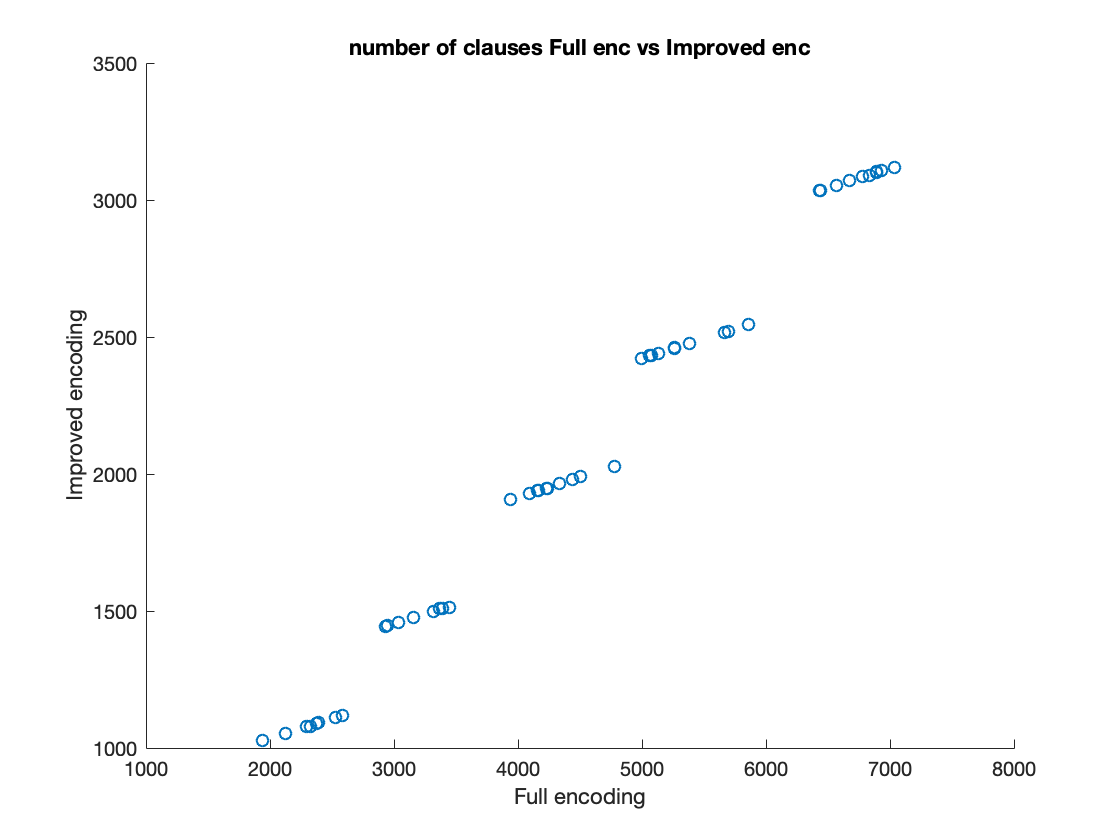
\includegraphics[width = 0.6\textwidth]{pic/clauses_e1vs2.png}
    \caption{The visualization of number of clauses generated by Simplified Full encoding and Improved encoding using Bayesian networks with deterministic ratio = 50. The most left cluster is 10 $\times$ 10}
    \label{fig:clauses_compare_1v2_r50}
\end{figure}

\begin{figure}
    \centering
    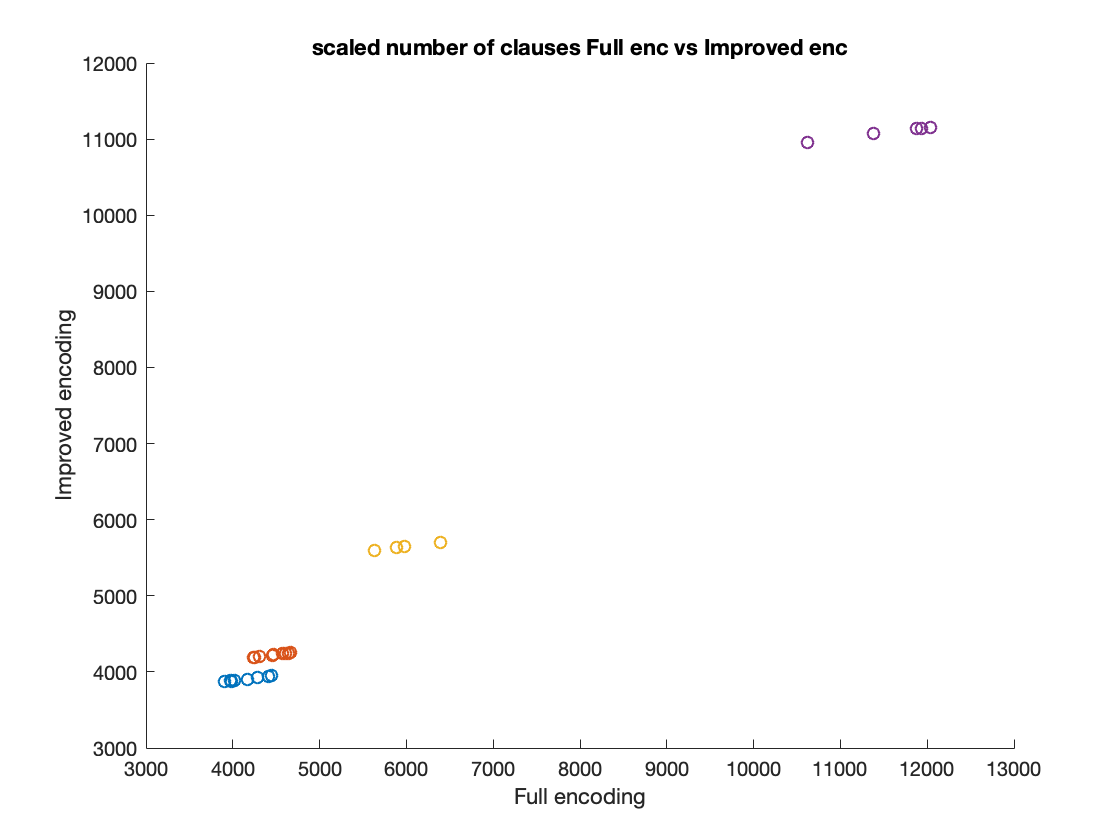
\includegraphics[width = 0.6\textwidth]{pic/r90_unscaled_clauses.png}
    \caption{The visualization of number of clauses generated by Simplified Full encoding and Improved encoding using Bayesian networks with deterministic ratio = 90. The most left cluster is 20 $\times$ 20}
    \label{fig:clauses_compare_1v2_r90}
\end{figure}

\begin{figure}
    \centering
    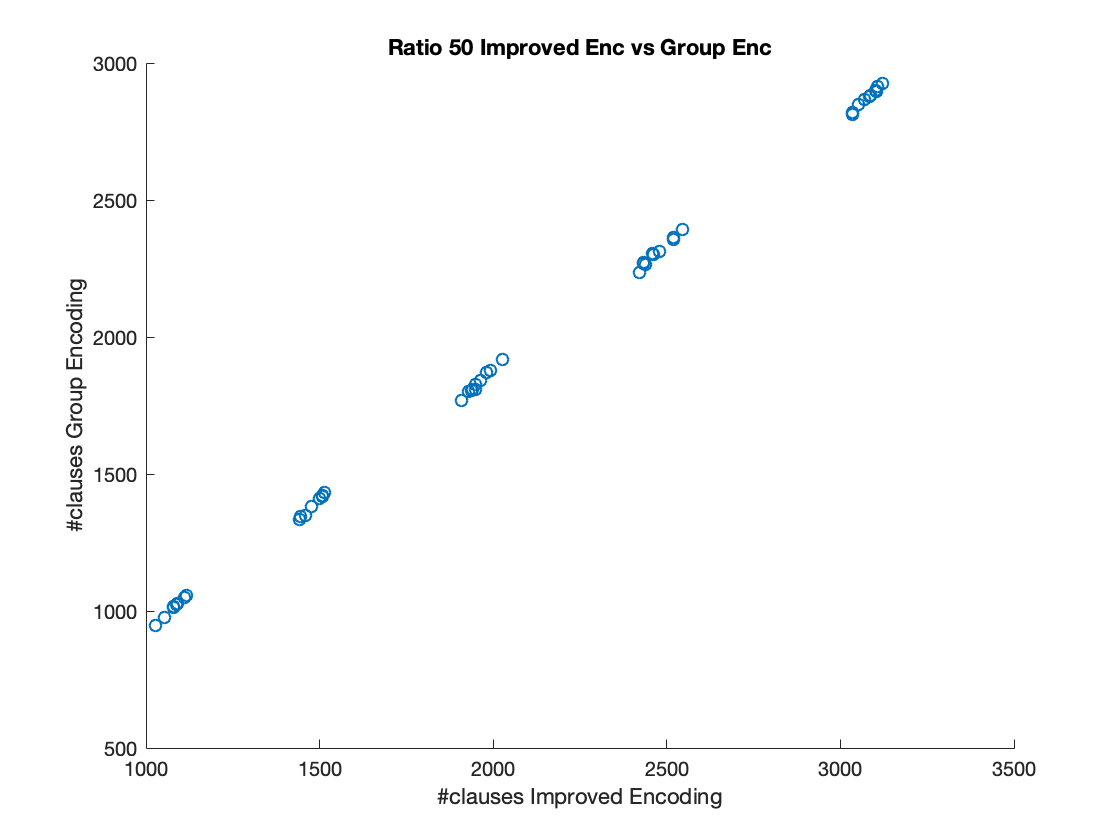
\includegraphics[width = 0.6\textwidth]{pic/r50_enc2v3.png}
    \caption{The visualization of number of clauses generated by Improved encoding and Group Encoding using Bayesian networks with deterministic ratio = 50}
    \label{fig:clauses_compare_2v3_r50}
\end{figure}

\begin{figure}
    \centering
    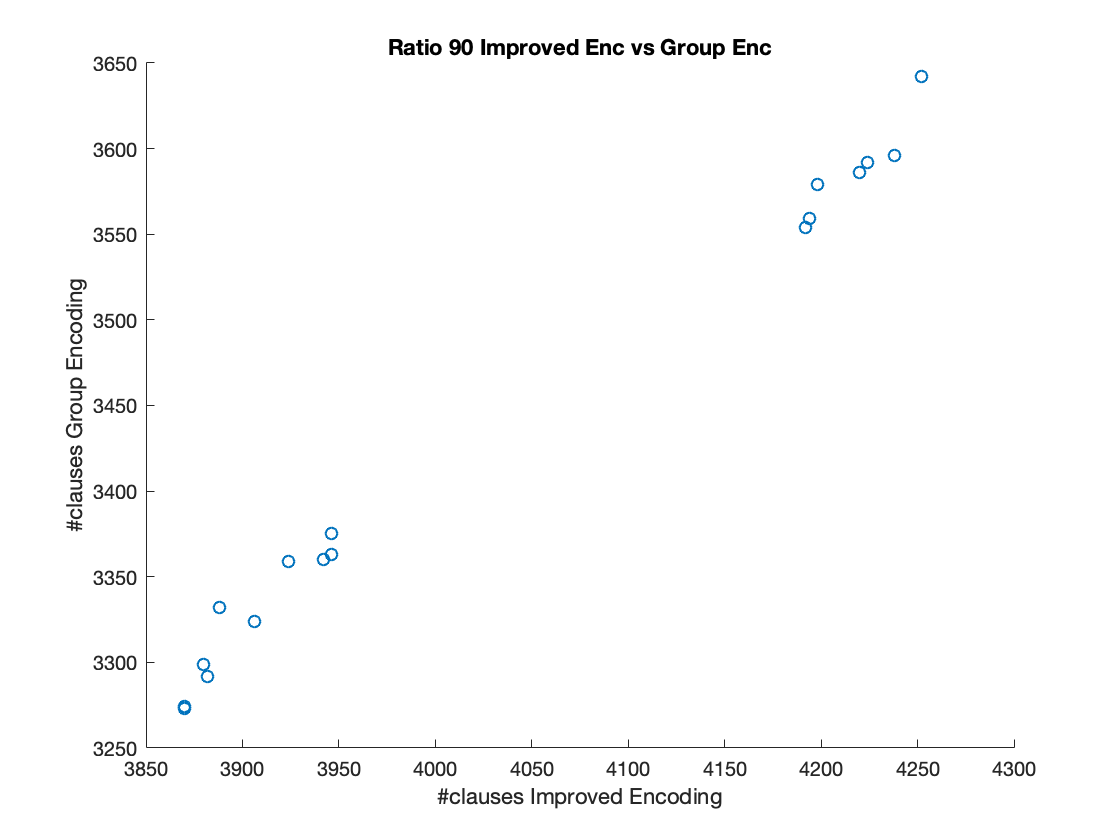
\includegraphics[width = 0.6\textwidth]{pic/r90_enc2v3.png}
    \caption{The visualization of number of clauses generated by Improved encoding and Group Encoding using Bayesian networks with deterministic ratio = 90}
    \label{fig:clauses_compare_2v3_r90}
\end{figure}

\noindent Figure \ref{fig:clauses_compare_1v2_r50} and Figure \ref{fig:clauses_compare_1v2_r90} are the visualisation of the number of clauses generate by Simplified Full encoding and Improved Encoding using network with deterministic ratio 50 and 70. Surprisingly, Grid Networks with certain deterministic ratio tends to have the same slope when comparing Simplified Full Encoding and Improved Encoding. In our case, the slope here was around 0.142. This result shows that from Simplified Full encoding to Improved Encoding, the reduction on the number of clauses generated is quite stable.\\

\noindent Figure \ref{fig:clauses_compare_2v3_r50} and  \ref{fig:clauses_compare_2v3_r90} visualize the reduction of clauses from Improved Encoding and Group Encoding. There was also a stable reduction in the number of clauses.


\begin{table}[]
    \centering
    \begin{tabular}{c c c c c}
    \hline
    &	    			&	Simplified Enc	&	Improved Enc	&	Group Enc	\\
    &	Network			&	Num Clauses	&	Num Clauses	&	Num Clauses	\\
    \hline
    \hline
	&	12	-	1	&	2126	&	1052	&	976	\\
	&	14	-	2	&	3158	&	1476	&	1380	\\
Ratio 50	&	16	-	1	&	4156	&	1938	&	1804	\\
	&	18	-	3	&	5260	&	2458	&	2305	\\
	&	20	-	1	&	6428	&	3034	&	2819	\\
	\hline
	&	10	-	1	&	918	&	644	&	568	\\
	&	10	-	2	&	1048	&	662	&	594	\\
	&	10	-	3	&	1030	&	660	&	600	\\
	&	12	-	1	&	1452	&	954	&	849	\\
	&	12	-	2	&	1422	&	948	&	847	\\
Ratio 75	&	12	-	3	&	1608	&	974	&	876	\\
	&	14	-	1	&	1614	&	1252	&	1087	\\
	&	14	-	2	&	1818	&	1280	&	1131	\\
	&	14	-	3	&	1894	&	1292	&	1138	\\
	&	15	-	3	&	2240	&	1496	&	1328	\\
	&	16	-	3	&	2612	&	1714	&	1512	\\
	\hline
	&	10	-	2	&	618	&	600	&	519	\\
	&	12	-	2	&	944	&	878	&	746	\\
	&	14	-	2	&	1238	&	1196	&	1021	\\
	&	15	-	2	&	1742	&	1422	&	1243	\\
Ratio 90	&	16	-	2	&	1338	&	1528	&	1289	\\
	&	17	-	2	&	2074	&	1810	&	1571	\\
	&	18	-	2	&	2080	&	1998	&	1711	\\
	&	19	-	2	&	2552	&	2264	&	1935	\\
	&	20	-	2	&	2686	&	2492	&	2148	\\
	\hline
	\hline
    \end{tabular}
    \caption{A Comparison of number of clauses generated by Simplified encoding, Improved encoding, and Group Encoding}
    \label{tab:comparing the clauses}
\end{table}

\subsection{Maximum Cluster Size}
The first analysis is based on the maximum cluster size of the tree. According to \cite{2008-literature-review}, this number is important because through exploiting topological structure for probabilistic inference run in time that is exponential in the maximum cluster size of the tree. Table \ref{tab:treesize} list the results of some benchmarks. The results showed that by encoding deterministic, weighted model counting method could successfully generate results in a reasonable amount of time even the size of the cluster is large. \\

\begin{table}[]
    \centering
    \begin{tabular}{l|c c c}
	\hline
   Benchmark					&	Max cluster size	&	Compie Time	&	NNF Memory (MB)	\\
   \hline
   \hline
    Ratio 50	-	10	-	1	&	30	&	0.142	&	5.5	\\
    Ratio 50	-	12-	1	&	36	&	0.694	&	26.5	\\
    Ratio 50	-	12	-	10	&	36	&	1.288	&	152.6	\\
    Ratio 75	-	10	-	1	&	30	&	0.013	&	0.48	\\
    Ratio 75	-	10	-	5	&	30	&	0.025	&	0.6706	\\
    Ratio 75	-	14	-	1	&	42	&	0.067	&	1.8	\\
    Ratio 75	-	18	-	5	&	52	&	32.199	&	671.9	\\
        \hline
    \end{tabular}
    \caption{Demonstrate the Effectiveness of using Weighted Model Counting method}
    \label{tab:treesize}
\end{table}

\subsection{Size of the NNF}
We then compare the file size generated in the model counter for the three encoding schemes. \\

\noindent During the model counting process, CNFs are first compiled into NNF format, and the file is stored with a .nnf extension. The compiled form support different Bayesian inference queries to be answered as many times as wanted. It has been shown in \cite{2008-literature-review} that given the same NNF, the variance of time used to solve different queries are small. So the Model counting time is used to represent the time used for Bayesian inference queries.\\

\noindent Table \ref{tab:size compare} compares the size of the NNF file in MegaBytes. Comparing the second and third column, observed that in general, from Simplified full encoding to Improved Encoding, the file size increase, sometimes twice as big as the size of Simplified encoding.
The larger file size also explained the reason why model counting time is longer for Improved Encoding.\\

\noindent Scatter plot in Figure \ref{fig:filesize_enc1v2} and Figure  \ref{fig:fullsize_enc1v3} shows respectively the compiled NNF sizes obtained by the miniC2D compiler. The visualization of the result shows that in most cases, the size of compiled NNF with Improved Encoding is the largest among all the encoding schemes, while the NNF file size of Group encoding became smaller than the ones generated by Improved encoding.

\begin{table}[]
    \centering
    \begin{tabular}{c|c c c}
    \hline
    Benchmark	&	Simp. Size (MB)	&	Impr. Size(MB)	&	Group. Size (MB)	\\
    \hline
    \hline
    12	-	1	&	19.13	&	34.93	&	11.00	\\
    12	-	2	&	30.43	&	28.30	&	10.53	\\
    12	-	3	&	30.13	&	34.47	&	21.60	\\
    12	-	4	&	28.80	&	52.87	&	21.83	\\
    12	-	5	&	22.00	&	35.00	&	32.40	\\
    14	-	2	&	43.30	&	85.63	&	31.93	\\
    14	-	4	&	142.37	&	199.87	&	52.03	\\
    14	-	5	&	197.93	&	315.23	&	69.23	\\
    14	-	6	&	59.07	&	99.80	&	26.57	\\
    14	-	7	&	319.10	&	389.10	&	173.60	\\
    16	-	1	&	327.90	&	383.53	&	264.70	\\
    16	-	2	&	736.83	&	1604.07	&	784.00	\\
    16	-	3	&	464.43	&	1003.77	&	138.43	\\
    16	-	4	&	945.03	&	1383.47	&	319.07	\\
    16	-	5	&	731.33	&	705.90	&	313.10	\\
    \hline
    \end{tabular}
    \caption{Comparing the size of the NNF file generated from the miniC2D model counter. The input is the encoded CNF using Simplified Full encoding, Improved encoding, and Group Encoding}
    \label{tab:size compare}
\end{table}

\begin{figure}
    \centering
    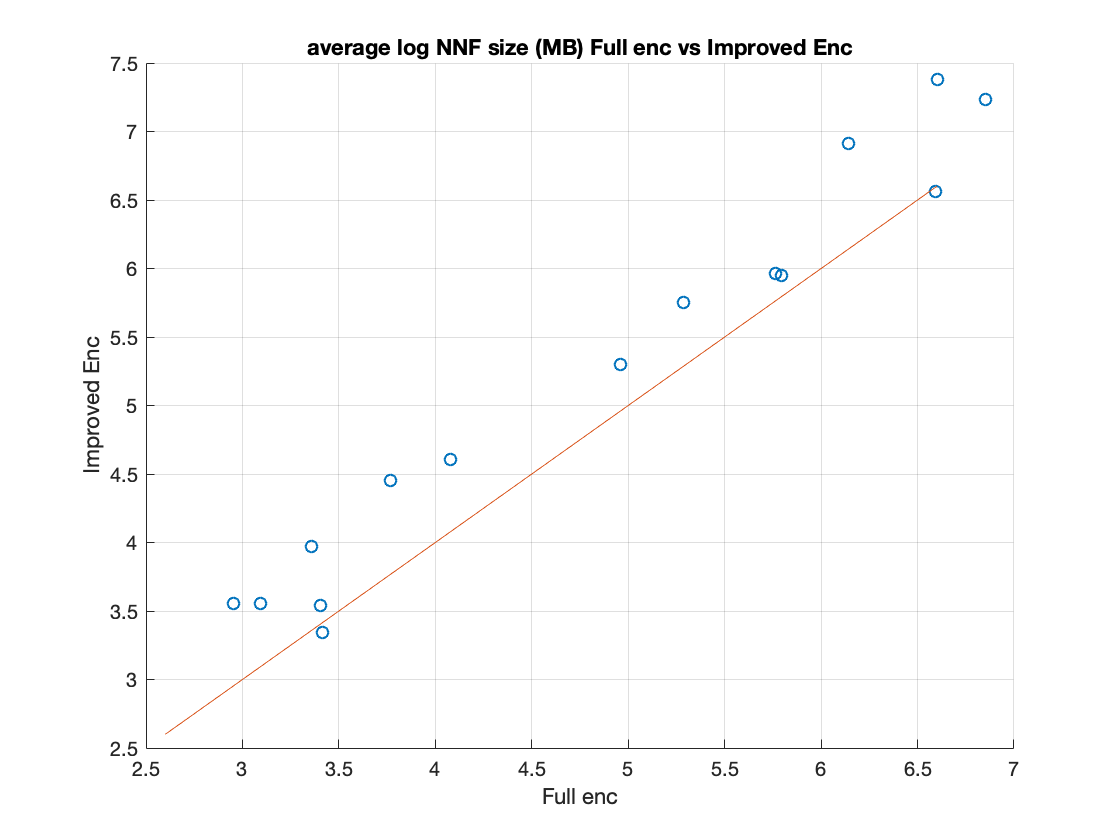
\includegraphics[width = 0.7 \textwidth]{pic/Size_fullvsImproved.png}
    \caption{NNF file size Simplified Full Enc vs Improved Enc}
    \label{fig:filesize_enc1v2}
\end{figure}

\begin{figure}
    \centering
    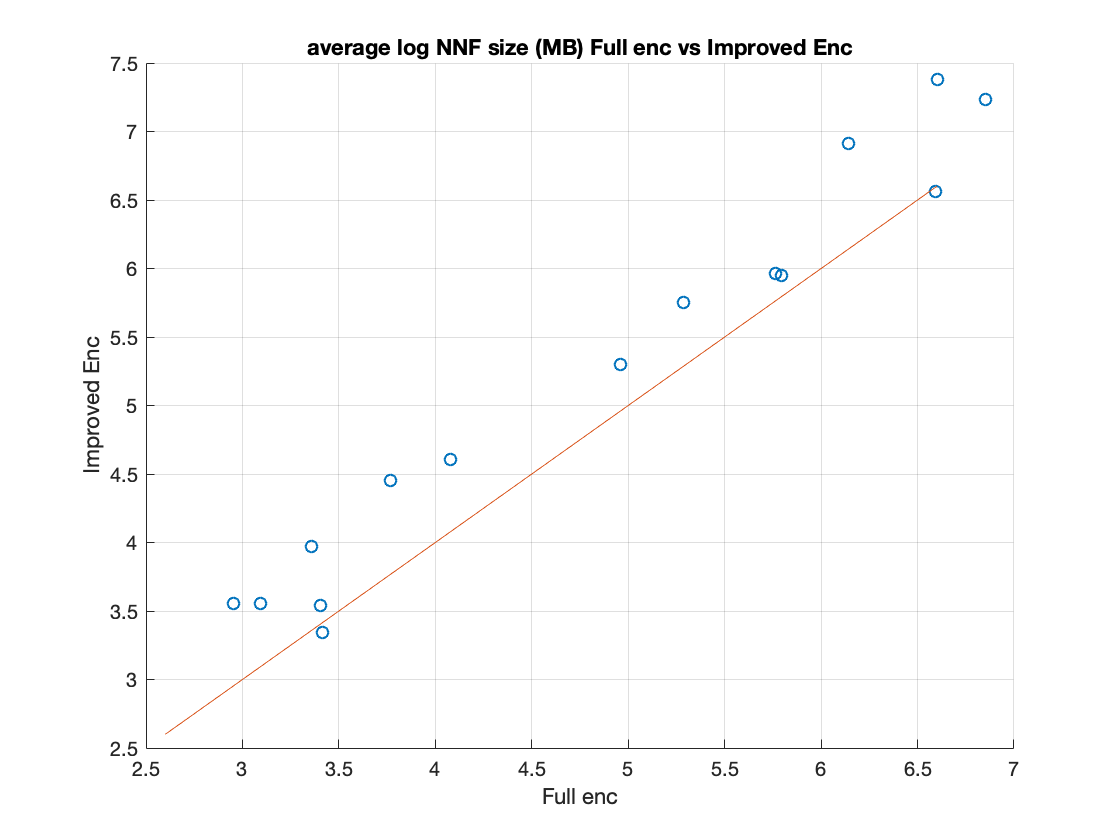
\includegraphics[width = 0.7 \textwidth]{pic/Size_fullvsImproved.png}
    \caption{NNF file size Simplified Full Enc vs Group Enc}
    \label{fig:fullsize_enc1v3}
\end{figure}

\subsection{Compling time and Counting time}
\begin{table}[]
    \centering
    \begin{tabular}{ c | c c | c c | c c}
    \hline
    	    	&	Simp.	&		&	Impr. 	&	 &	Group	&		\\
   		Bench	&	Comp.	&	Count.	&	Comp. 	&	Count. &	Comp. 	&	Count.	\\
   		mark		&	time	&	time	&	time	&time	& time	&	time	\\
   	\hline
   	\hline
12	-	1	&	3.51	&	0.32	&	1.14	&	0.52	&	0.27	&	0.14	\\
12	-	2	&	5.05	&	0.55	&	1.14	&	0.37	&	0.28	&	0.14	\\
12	-	3	&	3.43	&	0.47	&	1.33	&	0.43	&	0.54	&	0.31	\\
12	-	4	&	2.23	&	0.46	&	1.96	&	0.68	&	0.54	&	0.28	\\
12	-	5	&	2.37	&	0.35	&	1.15	&	0.44	&	0.76	&	0.46	\\
14	-	2	&	5.48	&	0.68	&	3.43	&	1.25	&	0.90	&	0.50	\\
14	-	4	&	20.26	&	2.51	&	5.76	&	2.97	&	1.26	&	0.70	\\
14	-	5	&	109.74	&	3.70	&	8.10	&	4.39	&	1.99	&	1.05	\\
14	-	6	&	19.24	&	0.93	&	2.89	&	1.38	&	0.88	&	0.40	\\
14	-	7	&	26.50	&	5.74	&	12.27	&	5.60	&	4.25	&	2.84	\\
16	-	1	&	70.52	&	5.72	&	13.04	&	5.26	&	6.34	&	4.59	\\
16	-	2	&	75.09	&	13.49	&	52.42	&	26.44	&	33.17	&	12.07	\\
16	-	3	&	100.47	&	8.11	&	46.78	&	15.84	&	3.58	&	2.27	\\
16	-	4	&	96.44	&	16.40	&	47.56	&	22.33	&	8.52	&	3.66	\\
16	-	5	&	40.38	&	12.37	&	17.37	&	10.42	&	10.60	&	4.20	\\
	\hline
	\hline
    \end{tabular}
    \caption{A Comparison of Compiling time and Counting time with Simplified Encoding, Improved Encoding and Group Encoding Using Ratio 50 Bayesian Networks}
    \label{tab:comparing time}
\end{table}

\noindent Recall that from Simplified encoding to Improved encoding then to Group encoding, these encoding schemes tend to produce smaller CNFs. Comparing Simplified Full Encoding with Improved Encoding shows that the latter method consistently has shorter compiling time.  the extra amount of time to count models from the compiled file is much less than the time used to Compiling the CNF to NNF.\\

\noindent Comparing column 4 and column 6, the results showed that although a similar number of clauses are generated, the Group encoding tends to have much shorter compiling time. It was demonstrated in \cite{2006-enc3} that the Group encoding tends to create clauses that have a fewer occurrence of irrelevant variables which benefits both the compiling time and the model counting time. For some of the benchmarks in the experiment, both Simplified encoding and Improved encoding failed to generate results in the model counter while the Group encoding managed to answer inference queries within the time limit. Some of the results are shown in Table \ref{tab:good Group encoding}\\
\begin{table}[]
\centering
\begin{tabular}{c|c c | c c | c c}
    \hline
    	&	Simpl.	&		&	Improved	&		&	Group	&		\\
    
	Bench		&	Comp. 	&	Counting 	&	Comp. 	&	Counting 	&	Comp. 	&	Counting 	\\
mark	&	Time	&	Time	&	Time	&	Time	&	Time	&	Time	\\
	\hline
	\hline
    42	-	2	&	-	&	-	& 63.1533 &	77.3533	&	10.0803	&	0.38467	\\
    42	-	3	&	-	&	-	&	-	&	-	&	118.6946	&	18.7187	\\
    42	-	4	&	-	&	-	&	-	&	-	&	60.56634	&	10.57233	\\
    42	-	5	&	-	&	-	&	-	&	-	&	255.5615	&	49.5615	\\
    \hline
\end{tabular}
\caption{Some of the bench marks when Improved encoding fail but Group encoding success}
    \label{tab:good Group encoding}
\end{table}

\noindent The scatter plot in Figure \ref{fig:time_enc1v2} and Figure \ref{fig:time_enc2v3} compares the T(compiling)+T(counting). Figure \ref{fig:time_enc1v2} shows that among most of the benchmarks we are testing, although Improved encoding tends to spend more time in compiling CNFs into target NNF file, the total time is faster using Improved Encoding. Figure \ref{fig:time_enc2v3} shows Group encoding lead to further reduction in time used in the compiling and model counting.\\

\begin{figure}
    \centering
    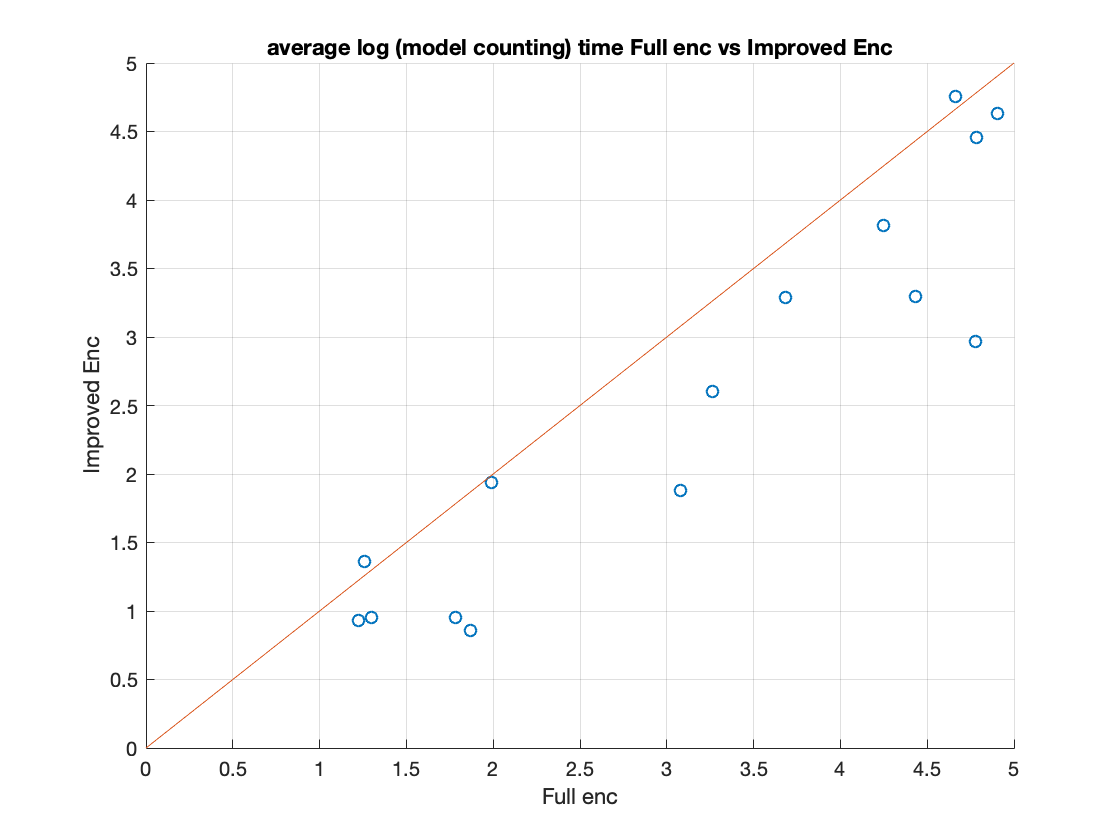
\includegraphics[width = 0.7 \textwidth]{pic/log_time_fullvsImproved.png}
    \caption{Comparing compiling time + counting time using Simplified Full encoding and Improved Encoding, The result take the logarithm of the time to fit the size of the figure}
    \label{fig:time_enc1v2}
\end{figure}

\begin{figure}
    \centering
    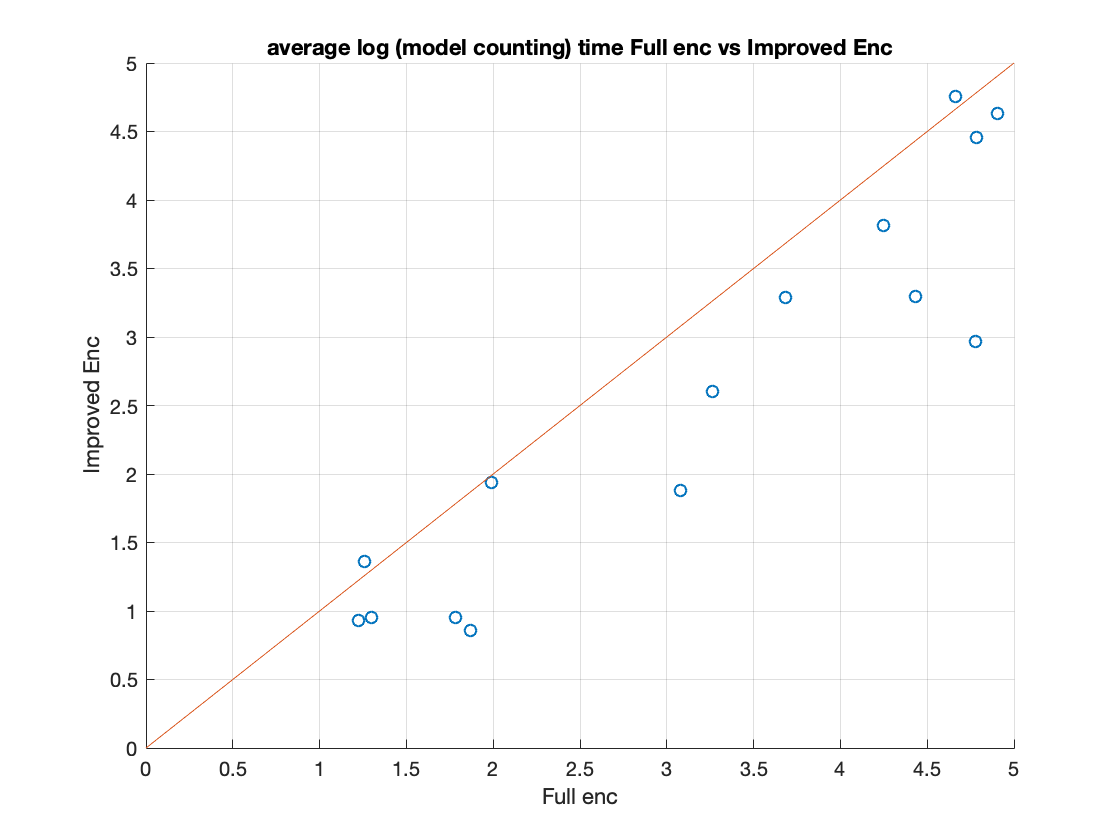
\includegraphics[width = 0.7 \textwidth]{pic/log_time_fullvsImproved.png}
    \caption{Comparing compiling time + counting time using Improved Encoding and Group Encoding. The result take the logarithm of the time to fit the size of the figure}
    \label{fig:time_enc2v3}
\end{figure}

\subsection{When Group encoding offers no advantages}
So far, concerning the number of clauses, compiling time and model counting time, Group encoding outperforms the other two encoding schemes. However, the run-time of the QM algorithm is exponential to the size of the input variables. When the Bayesian network nodes have a large number of parents, the QM algorithm won't be able to simplify the CNF within the time limit. Thus, the whole process fails during the encoding process.

\subsection{Comparing WMC with junction tree method}
Finally, we compared the weighted model counting method with the junction tree algorithm. The Junction tree algorithm here used the Pgmpy BeliefPropagation class. Table \ref{tab:junctree_vs_WMC} shows the result of using some of the benchmarks. When dealing with small networks that have a small number of nodes and sparsely connect, junction tree tends to generate results faster than the weighted model counting method. When the network became larger, the time used Junction tree grows significantly. However, although WMC method was slower when dealing with small networks, the time used by large networks was remarkably smaller.

\begin{table}[]
    \centering
    \begin{tabular}{c|c c c c}
        \hline
         Benchmark	&	Node numeber	&	Arc number	&	Junction tree	&	WMC	\\
         \hline
         \hline
        asia	&	8	&	8	&	0.04	&	0.2	\\
        caner	&	5	&	4	&	0.03	&	0.44	\\
        Earthquake	&	5	&	4	&	0.07	&	0.3	\\
        sachs	&	11	&	17	&	0.092	&	0.45	\\
        Hailfinder	&	56	&	66	&	90	&	14.9	\\
        Hepar	&	70	&	123	&	fail	&	0.53	\\
        Win95PTS	&	76	&	112	&	fail	&	50	\\
        Ratio50-10-1	&	100	&	-	&	fail	&	0.49	\\
        Ratio90-10-1	&	100	&	-	&	fail	&	0.42	\\
        \hline
    \end{tabular}
    \caption{Comparing Weighted Model Couning method using Improved Encoding and Junction Tree Algorithm}
    \label{tab:junctree_vs_WMC}
\end{table}

\subsection{Discussion of results}
In general, the Simplified full encoding generate the largest CNFs and have the longest model counting times, while the NNF file size after compiling the input CNF file is smaller compared to the Improved Encoding.\\

\noindent Improved encoding tends to generate smaller CNFs compared to Full encoding, and the total time spent in the model counting phase including compiling and counting tends to become shorter. While the file size might be more substantial and sometimes it will run out of memory. The size for a 16 $\times$ 16 Grid network with Ratio 50 determinism reached 2GB.\\

\noindent Group encoding outperforms both Simplified Full encoding and Improved encoding for the benchmarks with deterministic and small CPTs. It tends to have smaller CNF size, the shortest model counting time and small NNF file sizes. However, when it comes to Bayesian networks with large CPTs, the time spend on QM algorithm will grow exponentially, as a result, in those cases, the Group encoding won't perform well enough.

\subsection{Future work}
So far we have considered four encoding schemes that improved step by step. The log encoding we referred to based on the encoding scheme proposed in \cite{2016-logencoding} did further improvements build on the Group encoding, while due to the limit amount of time, we could not implement that encoding scheme. However, all of those encoding schemes focus on simplifying parameter clauses. The future work could find ways to simplify the indicator variables and indicator clauses. The project mainly focuses on the Encoding phase that is more algorithmic. It can be further integrated with the model counting software package combined with the user interface for large scale usage.